%===============================================================================
% $Id: ifacconf.tex 19 2011-10-27 09:32:13Z jpuente $  
% Template for IFAC meeting papers
% Copyright (c) 2007-2008 International Federation of Automatic Control
%===============================================================================
\documentclass[a4paper]{ifacconf}

\usepackage{graphicx,amsmath,url}      % include this line if your document contains figures
\usepackage[round]{natbib}             % required for bibliography
\usepackage{tabularx}                  % for tables
\usepackage{subcaption}                % for subplots
%===============================================================================


% ===============================================================
% Choose the language of the manuscript.
% If in English, choose 
% \def\portugues{0} 
%
% If in Portuguese or Spanish, choose
% \def\portugues{1} 
%
% Note that, if you are writing in Spanish, you need additional 
% adjusts in some parts of the text, which have been put in Portuguese only.
\def\portugues{1} 
% ===============================================================

% If the above line is commented, it is assumed manuscript in English:
\ifx\portugues\undefined
\def\portugues{0}
\fi


\if\portugues0
   \usepackage[english]{babel}
  \else
   \usepackage[spanish,brazil,english]{babel}
\fi

  

\usepackage[T1]{fontenc}
%\usepackage{inputenc}

\usepackage[utf8]{inputenc}

\usepackage{ae}


\if\portugues1
% =====================================================================
% =====================================================================
% If the manuscript is in Spanish, please change the texts adequatelly.
% You may also add other definitions in this part.
 \newtheorem{teorema}[thm]{{\em Teorema}}{ }
 \newtheorem{lema}[thm]{{\em Lema}}{ }
 \newtheorem{corolario}[thm]{{\em Corolário}}{ }
 \newenvironment{prova}{{\bf Prova.}}{ }
% ===============================================================
\fi

\begin{document}
	
	
\if\portugues1

% =====================================================================
% =====================================================================
% USE THIS PART IF THE TEXT IS IN PORTUGUES OR SPANISH
% =====================================================================
% If the manuscript is in Spanish, please change the texts adequately.
% =====================================================================
% 
\selectlanguage{brazil}
	
\begin{frontmatter}

\title{Calibração Automatizada de Analisador de Espectro Óptico para Faixa Visível via Visão Computacional} 
% Title, preferably not more than 10 words.

% \thanks[footnoteinfo]{Reconhecimento do suporte financeiro deve vir nesta nota de rodapé.}


\author[First]{A. Jakson} 
\author[Second]{N. João} 
\author[Third]{B. Felipe}
\author[Fourth]{B. Alexandre}

\address[First]{Faculdade de Engenharia Elétrica, Universidade Federal de Juiz de Fora, MG, (e-mail: jakson.almeida@estudante.ufjf.br).}
\address[Second]{Faculdade de Engenharia Elétrica, Universidade Federal de Juiz de Fora, MG, (e-mail: joao.nascimento@estudante.ufjf.br).}
\address[Third]{Faculdade de Engenharia Elétrica, Universidade Federal de Juiz de Fora, MG, (e-mail: felipe.barino@ufjf.br)}
\address[Fourth]{Faculdade de Engenharia Elétrica, Universidade Federal de Juiz de Fora, MG, (e-mail:alexandre.bessa@ufjf.br).}


\selectlanguage{english}
\renewcommand{\abstractname}{{\bf Abstract:~}}
\begin{abstract}                % Abstract of not more than 250 words.
This work presents the development of a low-cost Optical Spectrum Analyzer (OSA) for visible light spectra (380–750 nm), combining a 3D-printed spectrometer ("Osinha") and custom software ("OSA Visível"). The calibration process employs computer vision techniques to map wavelength-to-pixel relationships using white light and laser sources (532 nm and 650 nm). Key steps include centroid calculation, intensity thresholding, and linear regression via OpenCV and Pillow libraries. The software achieves a calibration accuracy of ±1.8 nm, validated through experiments with controlled light sources. By reducing costs from over \$30 000 (commercial OSA) tounder \$200, this solution democratizes spectral analysis for educational and research applications. The intuitive interface allows real-time visualization and data export, eliminating the need for specialized programming skills.

\vskip 1mm% não altere esse espaçamento
\selectlanguage{brazil}
{\noindent \bf Resumo}:  Este trabalho apresenta o desenvolvimento de um Analisador de Espectro Óptico (OSA) de baixo custo para a faixa visível (380–750 nm), combinando um espectrômetro impresso em 3D ("Osinha") e um software customizado ("OSA Visível"). O processo de calibração emprega técnicas de visão computacional para mapear a relação comprimento de onda-posição de pixel, utilizando luz branca e lasers (532 nm e 650 nm). Etapas-chave incluem cálculo de centróide, limiarização de intensidade e regressão linear via bibliotecas OpenCV e Pillow. O software atinge precisão de ±1.8 nm, validada em experimentos com fontes de luz controladas. Ao reduzir custos de mais de \$30 000 (OSA Comercial) para menos de \$200, esta solução democratiza a análise espectral para aplicações educacionais e de pesquisa. A interface intuitiva permite visualização em tempo real e exportação de dados, dispensando conhecimentos em programação.
\end{abstract}

\selectlanguage{english}


\begin{keyword}
Optical Spectrum Analyzer; Automated calibration; Computer vision; Visible spectrum; Linear regression.

\vskip 1mm% não altere esse espaçamento
\selectlanguage{brazil}
{\noindent\it Palavras-chaves:} Analisador de Espectro Óptico; Calibração automatizada; Visão computacional; Espectro visível; Regressão linear.
\end{keyword}


\selectlanguage{brazil}


\end{frontmatter}
\else
% ===============================================================
% ===============================================================
% USE THIS PART IF THE TEXT IS IN ENGLISH
% ===============================================================
% ===============================================================
% 

\begin{frontmatter}

\title{Style for SBA Conferences \& Symposia: Use Title Case for
  Paper Title\thanksref{footnoteinfo}} 
% Title, preferably not more than 10 words.

\thanks[footnoteinfo]{Sponsor and financial support acknowledgment
goes here. Paper titles should be written in uppercase and lowercase
letters, not all uppercase.}

\author[First]{First A. Author} 
\author[Second]{Second B. Author, Jr.} 
\author[Third]{Third C. Author}


\address[First]{Faculdade de Engenharia Elétrica, Universidade do Triângulo, MG, (e-mail: autor1@faceg@univt.br).}
\address[Second]{Faculdade de Engenharia de Controle \& Automação, Universidade do Futuro, RJ (e-mail: autor2@feca.unifutu.rj)}
\address[Third]{Electrical Engineering Department, 
   Seoul National University, Seoul, Korea, (e-mail: author3@snu.ac.kr)}
   
\renewcommand{\abstractname}{{\bf Abstract:~}}   
   
\begin{abstract}                % Abstract of not more than 250 words.
These instructions give you guidelines for preparing papers for IFAC
technical meetings. Please use this document as a template to prepare
your manuscript. For submission guidelines, follow instructions on
paper submission system as well as the event website.
\end{abstract}

\begin{keyword}
Five to ten keywords, preferably chosen from the IFAC keyword list.
\end{keyword}

\end{frontmatter}
\fi

%===============================================================================
%===============================================================================
%===============================================================================


\section{Introdução}

Analisadores de Espectro Óptico (OSA) comerciais que operam na faixa visível apresentam custos elevados\footnote{Pesquisa realizada em março de 2025. Para mais detalhes sobre os preços de OSAs comerciais, consulte a Tabela \ref{tab:market}.}, frequentemente superiores a \$30.000, conforme \cite{OSA201C}. Isso restringe o uso desses equipamentos para muitas instituições acadêmicas e laboratórios de pequeno porte. Como alternativa, o "Osinha" foi desenvolvido com uma abordagem de baixo custo, utilizando impressão 3D, uma webcam e uma grade de difração, totalizando menos de \$200 USD, tornando-o uma solução acessível para pesquisa e ensino.


Este trabalho propõe uma solução de baixo custo baseada em hardware aberto ("Osinha") e software customizado ("OSA Visível"), desenvolvido pelo Laboratório de Instrumentação e Telemetria (LITel/UFJF). O diferencial reside no uso de técnicas de visão computacional para calibração automática, substituindo métodos manuais ou baseados em hardware dedicado.

A calibração combina duas etapas: (i) captura do espectro contínuo de luz branca, com detecção do centróide e ajuste inicial de uma reta via regressão linear; e (ii) correlação direta entre picos de intensidade de lasers (532 nm e 650 nm) e suas posições na imagem, definindo a relação comprimento de onda-posição de pixel.

Este artigo está organizado da seguinte forma: a Seção 2 detalha a metodologia de calibração; a Seção 3 descreve o desenvolvimento do software; a Seção 4 valida os resultados experimentais; e a Seção 5 discute conclusões e trabalhos futuros.

\section{METODOLOGIA}
\label{sec:metodologia}

\subsection{Base teórica e trabalhos correlatos}
A calibração de analisadores de espectro óptico (OSA) para a faixa visível tem sido amplamente explorada na literatura. \cite{dubard1995} discutiram a necessidade de caracterizar com precisão as fontes ópticas em medições de fibras ópticas e apresentaram técnicas de calibração para OSAs. Abordagens modernas, \cite{liu2013} empregam métodos de calibração precisos utilizando parâmetros do sistema para espectrômetros de grade. Alternativamente, \cite{terra2015} propuseram três métodos para calibrar um OSA baseado em grade, utilizando fontes laser bem caracterizadas, duplicação de frequência em cristais não lineares e uma célula de gás de cianeto de hidrogênio como referência de comprimento de onda. Neste trabalho, adota-se uma estratégia híbrida: a calibração inicial com luz branca fornece uma relação linear preliminar, enquanto lasers de referência (532 nm e 650 nm) definem a escala absoluta, combinando assim simplicidade e baixo custo — uma lacuna não abordada pelos métodos existentes.

A Tabela \ref{tab:market} destaca os altos custos de OSAs comerciais (e.g., \cite{thorlabs_osa20xc}, \cite{anritsu_ms9740b}), justificando o desenvolvimento de uma solução acessível (OSA Visível).

\begin{table}[hb]
\begin{center}
\caption{Preços e especificações de OSA comerciais (dados de março de 2025).}\label{tab:market}
\begin{tabular}{>{\raggedright\arraybackslash}p{2.5cm}>{\centering\arraybackslash}p{2cm}>{\centering\arraybackslash}p{2.5cm}>{\raggedright\arraybackslash}p{2cm}}
Modelo (Marca) & Faixa Espectral (nm) & Preço (USD) \\\hline
OSA201C \cite{thorlabs_osa20xc} & 350–1100 & 30.767,19 \\
AQ6380 \cite{yokogawa_aq6374} & 350–1750 & 100.000–200.000 \\
MS9740B \cite{anritsu_ms9740b} & 600–1750 & 20.000–40.000 \\
OSA Visível (Osinha) & 380–750 & <200 \\ \hline
\end{tabular}
\end{center}
\end{table}

\subsection{Arquitetura do hardware}
O hardware do espectrômetro "Osinha" (Fig. \ref{fig:osinha}) foi desenvolvido com base no projeto \textit{Open Fiber Spectrometer} \cite{gaudi_spectrometer}, um espectrômetro de código aberto que fornece modelos 3D e instruções detalhadas para construção. O projeto original foi adaptado para atender às necessidades específicas deste trabalho, com foco na faixa visível do espectro (380–750 nm). 

O hardware consiste nos seguintes componentes principais:
\begin{itemize}
    \item Grade de difração ($1000 \cdot \text{linhas} / \text{mm}$): relação comprimento de onda ($\lambda$)-ângulo de difração ($\theta$), \cite{fraunhofer}, dada por:
    \begin{equation}
        n\lambda = d(\sin\theta + \sin\alpha)
        \label{eq:diffraction}
    \end{equation}
    onde $d = 1\,\mu\text{m}$ (espaçamento da grade), $n$ (ordem de difração), $\alpha$ (ângulo de incidência).
    
    \item Webcam USB: resolução de $640 \times 480$ pixels, taxa de amostragem de $30$ fps. O sinal digital é discretizado como:
    \begin{equation}
        I(x,y) = \sum_{k=0}^{255} k \cdot P(k|x,y)
        \label{eq:sampling}
    \end{equation}
    onde $P(k|x,y)$ é a probabilidade do pixel $(x,y)$ ter intensidade $k$.
\end{itemize}

\begin{figure}[ht]
\centering
\includegraphics[width=0.5\textwidth]{data/Osinha - PAPER.png}
\caption{Espectrômetro Osinha: (1) Luz incidente, (2) Fenda óptica, (3) Grade de difração, (4) Webcam. Imagem ilustrativa, \cite{gaudi_spectrometer}.}
\label{fig:osinha}
\end{figure}

\subsection{Processo de Calibração}
\label{subsec:calibracao}

(1) Aquisição do Sinal Digital:

A calibração inicia com a captura de imagens em tempo real do espectrômetro via \textit{OpenCV}. Para a calibração com fonte de luz branca o processo se dá por um único quadro ($N=1$).

Para a calibração utilizando lasers, segunda etapa do processo, $N$ quadros ($N=20$) no intervalo homogêneo de tempo de 2 segundos são obtidos seus ganhos de intensidade para redução de ruído por meio de média aritmética:
\begin{equation}
    \bar{I}(x,y) = \frac{1}{N}\sum_{i=1}^{N} I_i(x,y)
    \label{eq:frame_avg}
\end{equation}

(2) Pré-processamento com Visão Computacional:

\begin{itemize}
    \item Conversão para escala de cinza:
    \begin{equation}
        I_{gray}(x,y) = \frac{R + G + B}{3}
    \end{equation}
    onde $R$, $G$ e $B$ são, respectivamente, as intensidades para os pixels vermelho, verde e azul.
    
    \item Segmentação por limiar adaptativo:
    \begin{equation}
        M(x,y) = \begin{cases}
            I_{gray}(x,y), & \text{se } I_{gray}(x,y) \geq T \\
            0, & \text{caso contrário}
        \end{cases}
        \label{eq:threshold}
    \end{equation}
    onde $T$ é determinado pelo método de Otsu \cite{otsu1979}.
\end{itemize}

(3) Regressão Linear para Mapeamento $\lambda$-pixel:

Para luz branca, calcula-se o centróide do espectro:
\begin{equation}
    x_c = \frac{\sum_{x,y} x \cdot M(x,y)}{\sum_{x,y} M(x,y)}, \quad
    y_c = \frac{\sum_{x,y} y \cdot M(x,y)}{\sum_{x,y} M(x,y)}
    \label{eq:centroid}
\end{equation}

Após a segmentação por limiar adaptativo (Eq. \ref{eq:threshold}), os pixels ativos (\(M(x,y) \geq T\)) formam uma nuvem de pontos ao longo do espectro. A reta de regressão linear (\(y = m \cdot x + c\)) é obtida via método dos \textit{mínimos quadrados}, minimizando:  

\begin{equation}  
    \min_{m,c} \sum_{x,y} \left(y - (m \cdot x + c)\right)^2 
\end{equation}  

Os coeficientes \(m\) (inclinação) e \(c\) (intercepto) definem a orientação espacial do espectro. Combinado com o centróide (Eq. \ref{eq:centroid}), esta reta estabelece a relação preliminar \textit{posição de pixel} com \textit{comprimento de onda}, posteriormente ajustada pelos lasers.  


A relação \(\lambda(x) = a \cdot x + b\) é definida pelos pontos dos lasers:
\begin{equation}
    a = \frac{\lambda_{\text{verm}} - \lambda_{\text{verd}}}{x_{\text{verm}} - x_{\text{verd}}}, \quad  
    b = \lambda_{\text{verd}} - a \cdot x_{\text{verd}}
\end{equation}

onde \(\lambda_{\text{verd}} = 532\) nm e \(\lambda_{\text{verm}} = 650\) nm.

(4) Correlação com Lasers de Referência:

Dois lasers de comprimento de onda conhecido (Verde: 532 nm, Vermelho: 650 nm) são utilizados para mapear a posição de seus picos de intensidade na reta de calibração previamente ajustada. A partir das coordenadas \((x_{532}, 532)\) e \((x_{650}, 650)\), calcula-se a relação linear \(\lambda(x) = a \cdot x + b\), onde \(a\) e \(b\) são determinados pelos pontos fixos dos lasers.
A posição do pico é determinada por:
\begin{equation}
    x_{peak} = \arg \max_{x} \, I(x).
    \label{eq:peak}
\end{equation}

\begin{table}[ht]
    \centering
    \caption{Parâmetros de calibração obtidos experimentalmente}
    \label{tab:calib_params}
    \begin{tabular}{lcc}
        \toprule
        Parâmetro & Luz Branca & Lasers \\
        \hline
        \midrule
        Coeficiente $a$ (nm/pixel) & -0.0608250474 & 1.475 \\
        Coeficiente $b$ (nm) & 203.136815 & 195.7 \\
        Erro RMS (nm) & 2.1 & 1.8 \\
        \hline
        \bottomrule
    \end{tabular}
\end{table}

\subsection{Implementação do Algoritmo}
O fluxo de processamento do software OSA Visível é dividido em duas etapas principais: \textit{calibração com luz branca} e \textit{calibração com lasers}. As etapas são as seguintes:

\begin{itemize}
    \item Calibração com Luz Branca:
    \begin{itemize}
        \item Captura de um quadro do espectro contínuo via webcam (OpenCV).
        \item Pré-processamento da imagem: conversão para escala de cinza e limiarização adaptativa (método de Otsu).
        \item Cálculo do centróide do espectro (Eq. \ref{eq:centroid}).
        \item Regressão linear para ajuste preliminar da reta \(\lambda(x) = a \cdot x + b\).
        \item Salvamento dos parâmetros preliminares (coeficientes \(a\), \(b\), centroide).
    \end{itemize}
    
    \item Calibração com Lasers:
    \begin{itemize}
        \item Captura de 20 quadros para redução de ruído (média temporal).
        \item Detecção dos picos de intensidade dos lasers verde (532 nm) e vermelho (650 nm).
        \item Cálculo da posição \(x\) dos picos na imagem (OpenCV).
        \item Ajuste final da relação \(\lambda(x)\) usando os pontos fixos dos lasers.
        \item Validação da reta de calibração e atualização dos parâmetros \(a\) e \(b\).
    \end{itemize}
\end{itemize}

% \begin{figure}[ht]
%     \centering
%     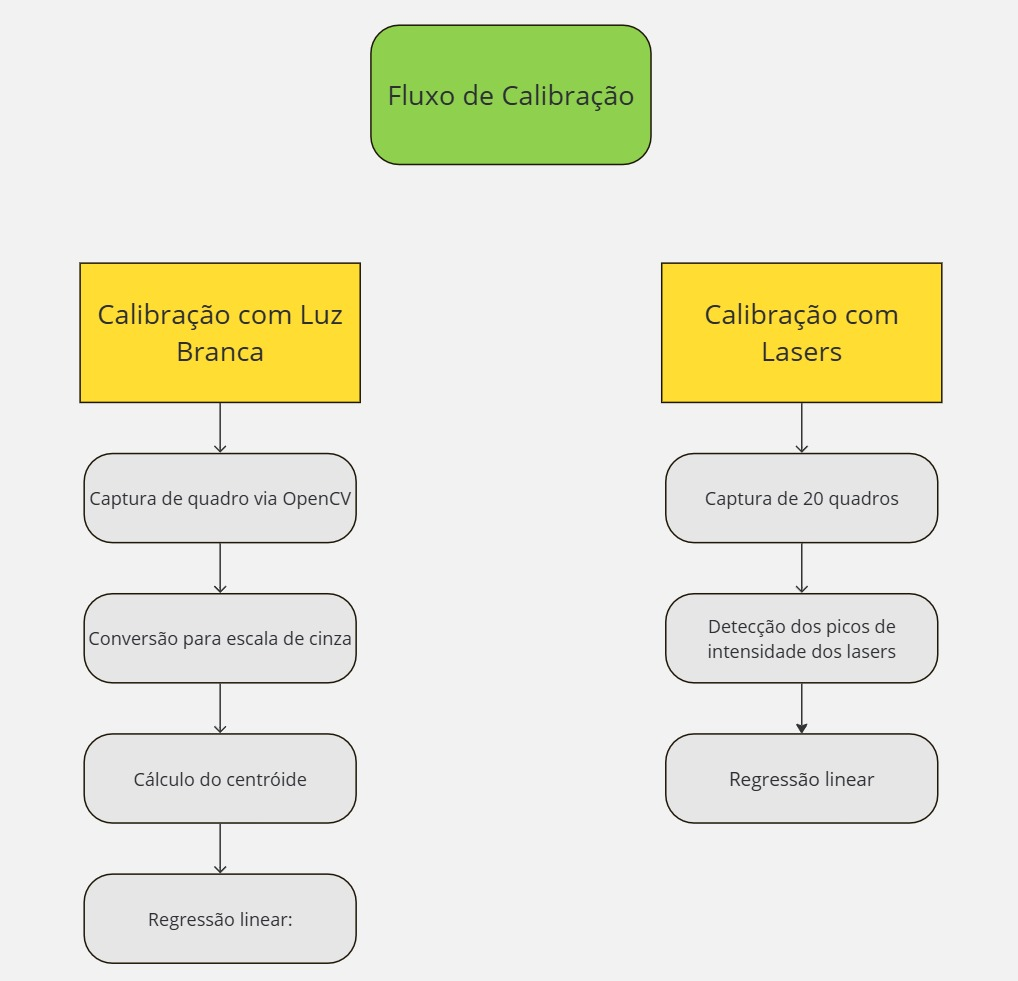
\includegraphics[width=0.4\textwidth]{data/flux1.jpg}
%     \caption{Fluxograma do processo de calibração do OSA Visível. A etapa de luz branca (azul) define a reta preliminar, enquanto os lasers (verde/vermelho) estabelecem a relação absoluta entre posição de pixel e comprimento de onda.}
%     \label{fig:fluxo}
% \end{figure}

\section{DESENVOLVIMENTO DO SOFTWARE}
\label{sec:software}

\subsection{Arquitetura e plataforma}
O software \textit{OSA Visível} foi desenvolvido em Python, utilizando a biblioteca \textit{Tkinter} para a interface gráfica, garantindo compatibilidade com Windows 10/11 e Linux Ubuntu 22.04. A escolha do Python deve-se à sua portabilidade e à vasta gama de bibliotecas para visão computacional (OpenCV, Pillow) e processamento numérico (NumPy, SciPy).

\subsection{Design da interface}

A interface foi projetada para guiar o usuário em um fluxo intuitivo, com dentre suas \textit{principais funcionalidades}:

\begin{itemize}
    \item Janela Principal (Fig. \ref{fig:gui}): Apresenta a visualização do espectro em tempo real, gráficos de intensidade ($I(\lambda)$) e comprimento de onda ($\lambda$), um widget de logs do sistema e botões de acesso rápido para calibração e configurações do sistema.
    \item Janela de Calibração: Oferece um assistente passo a passo (Fig. \ref{fig:calib_gui}), com as seguintes funcionalidades:
    \begin{itemize}
        \item Calibração automática para luz branca com um único clique.
        \item Guia interativo para calibração utilizando lasers.
        \item Visualização em tempo real do sinal digital da fonte de dados e da reta de regressão.
    \end{itemize}
    \item Janela de Configuração da Webcam: Permite a seleção entre webcams disponíveis e a utilização de vídeos previamente gravados como fonte de dados.
    \item Janela de Salvamento de Dados: Facilita a exportação de espectros em formato .txt e permite a programação de salvamentos periódicos dos espectros.
\end{itemize}

\begin{figure}[ht]
    \centering
    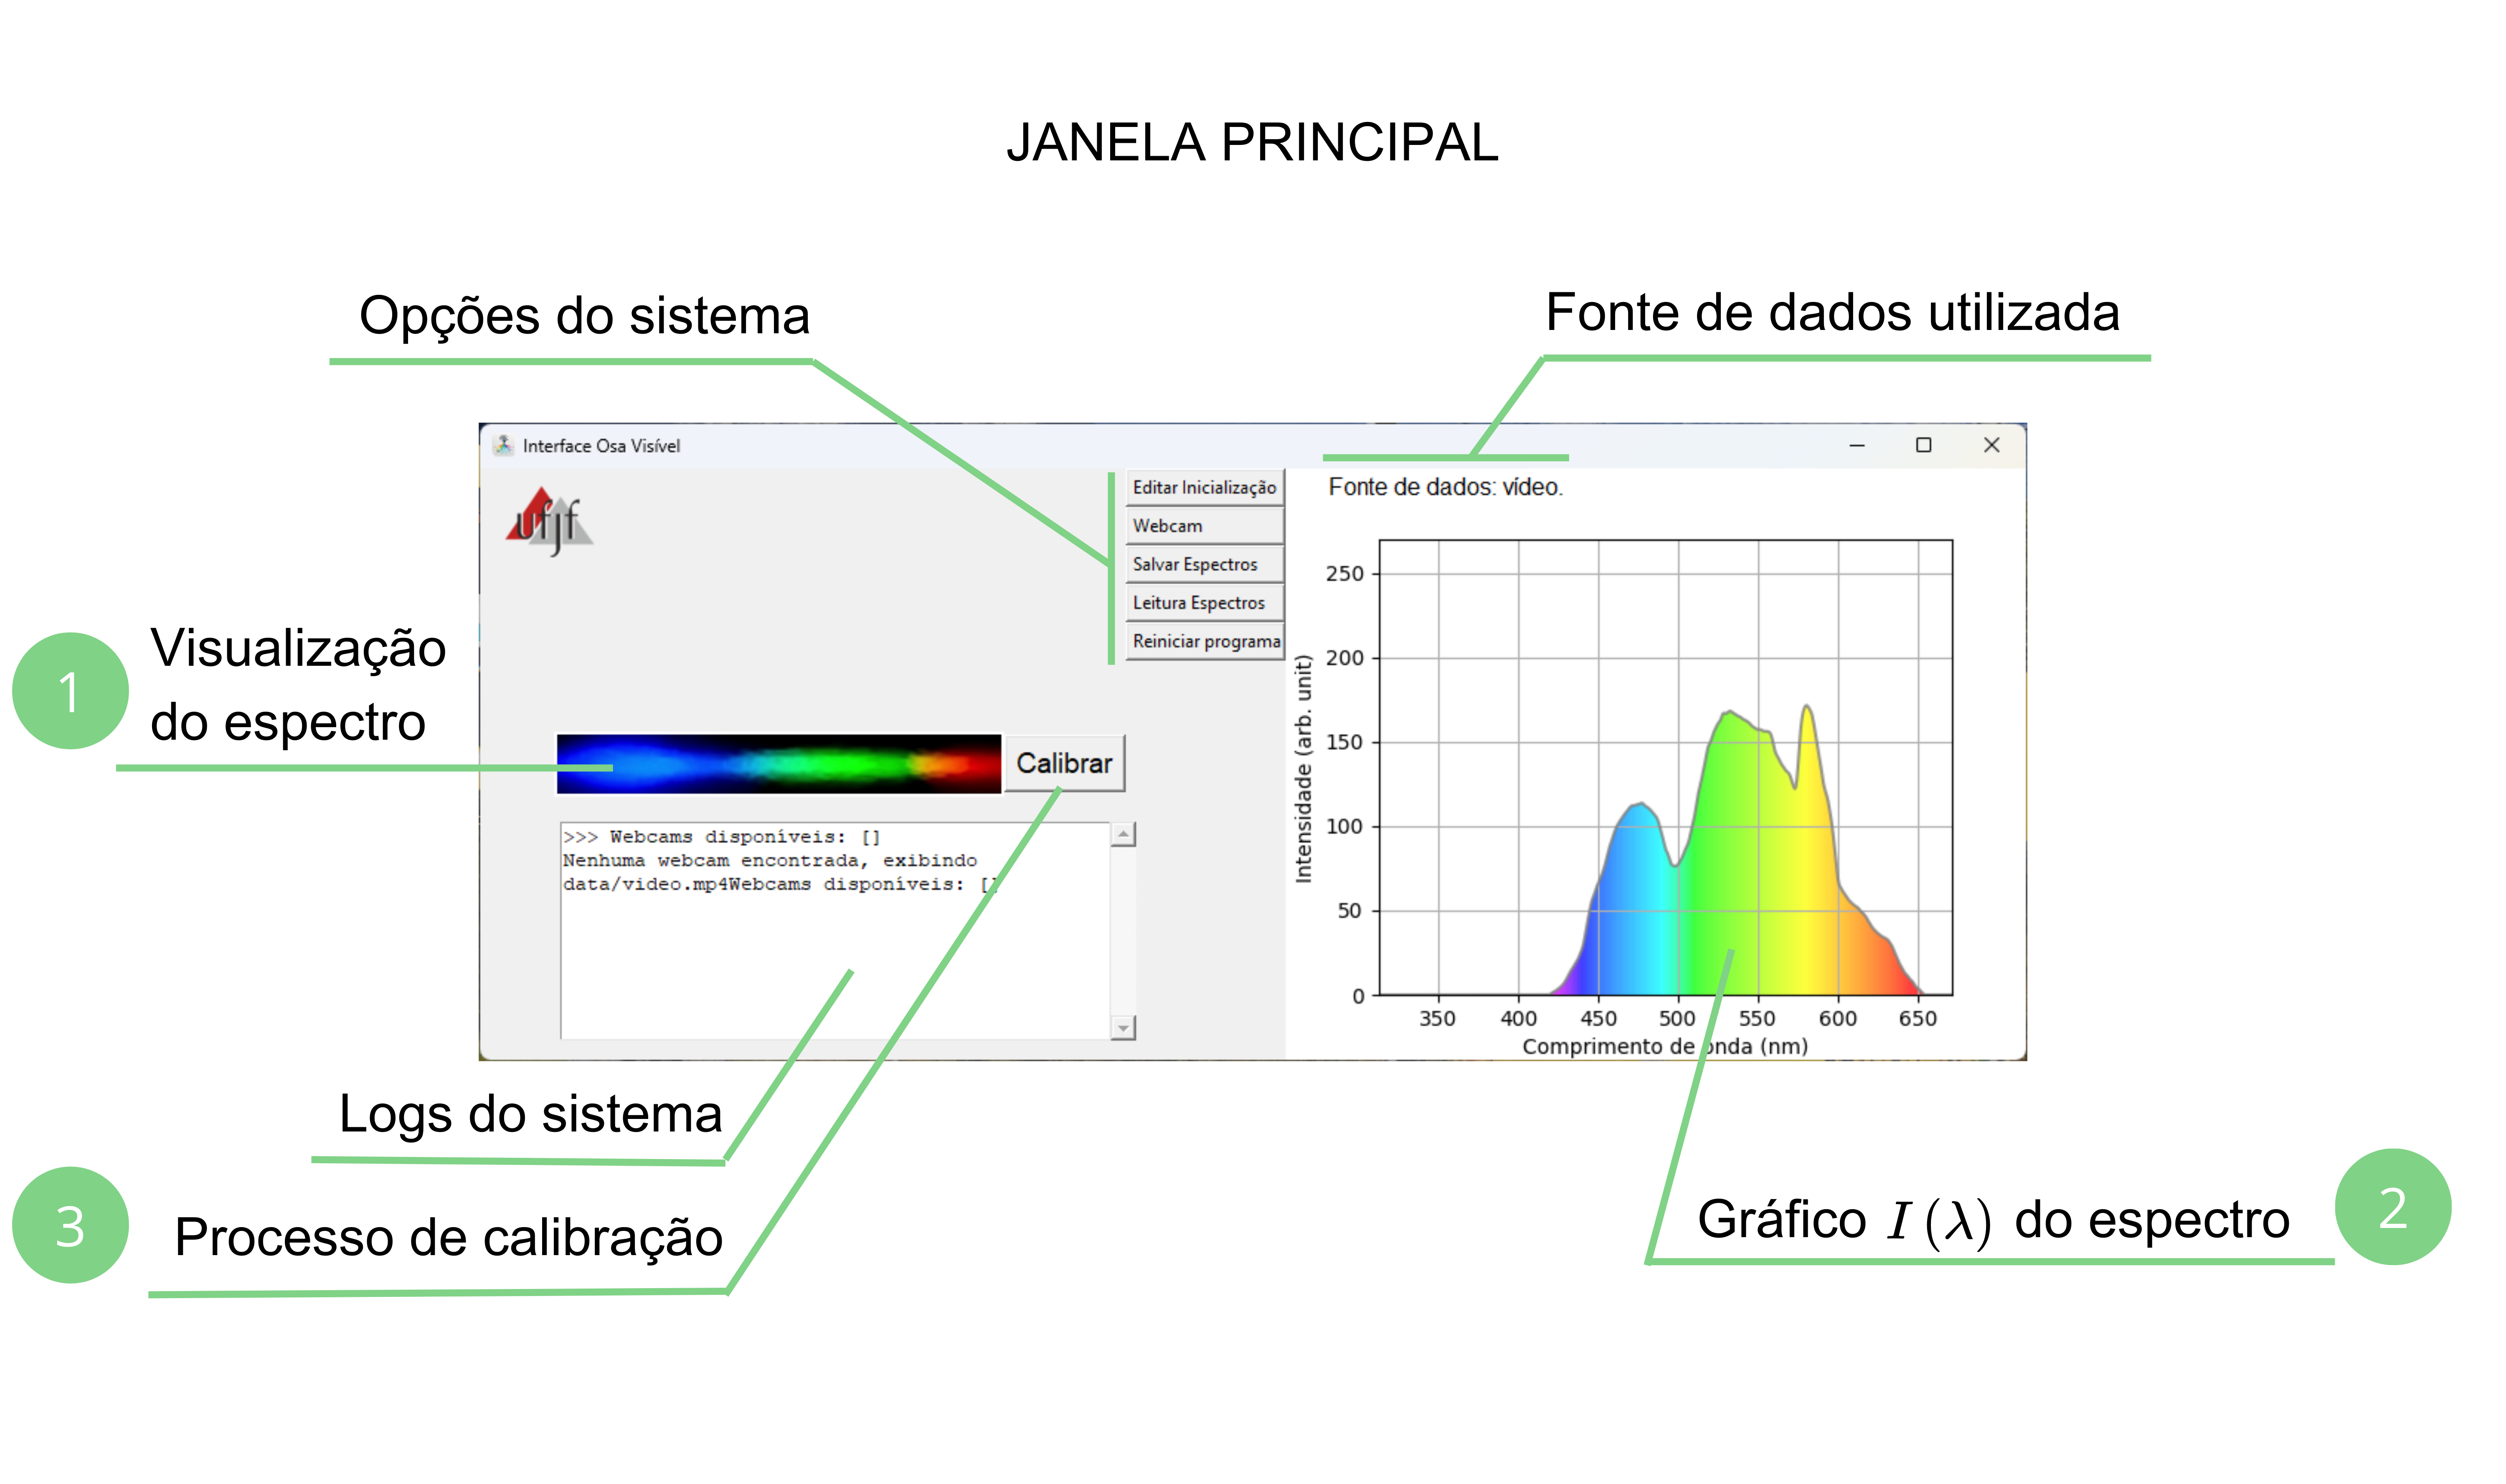
\includegraphics[width=0.5\textwidth]{data/janela_principal_recursos.png}
    \caption{Janela principal do OSA Visível: (1) Visualização do espectro, (2) Gráfico $I(\lambda)$ do espectro, (3) Processo de calibração do espectrômetro.}
    \label{fig:gui}
\end{figure}

\subsection{Processo de Calibração Passo a Passo}
\label{subsec:calib_software}
O fluxo de calibração automatizada inclui:
\begin{enumerate}
    \item Calibração com Luz Branca:
    \begin{itemize}
        \item Detecção do centróide via OpenCV (Eq. \ref{eq:centroid}).
        \item Cálculo dos coeficientes $a$ e $b$ da reta $\lambda(x)$.
    \end{itemize}
    
    \item Calibração com Lasers:
Após a calibração inicial com luz branca — que estabelece uma correlação linear entre a intensidade dos pixels e sua posição na imagem —, os lasers de referência são empregados para mapear essa reta aos comprimentos de onda conhecidos. 

Nesse processo:
\begin{itemize}
    \item Laser verde (532 nm) e laser vermelho (650 nm) são utilizados para identificar os picos de intensidade correspondentes.
    \item A posição dos picos na reta de calibração, obtida com a luz branca, é correlacionada com os comprimentos de onda reais dos lasers.
    \item Essa correspondência permite ajustar os parâmetros da reta de calibração, definindo a relação \(\lambda(x) = a \cdot x + b\), de modo a representar com precisão a relação entre os pixels e os comprimentos de onda.
\end{itemize}

Essa etapa garante que a calibração do sistema seja fundamentada em referências de comprimento de onda bem definidas.
\end{enumerate}

\begin{figure}[ht]
    \centering
    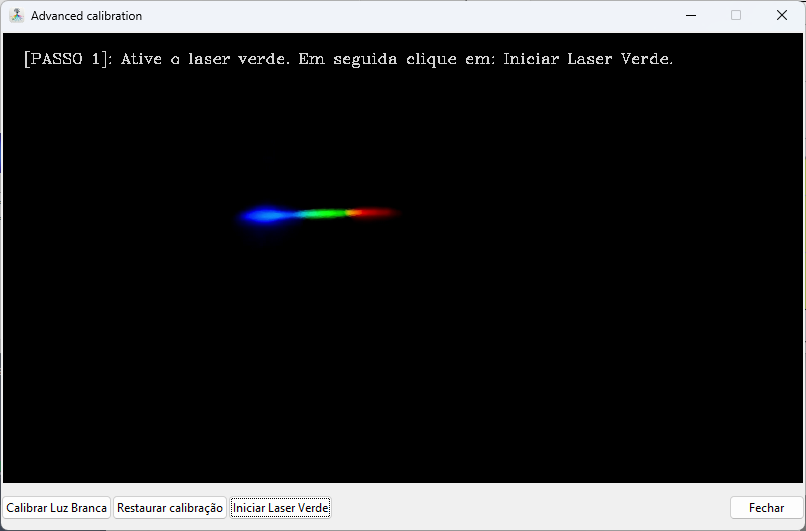
\includegraphics[width=0.4\textwidth]{data/calibration_window.png}
    \caption{Janela de calibração, principais recursos: (1)\textit{ Calibrar Luz Branca}: calibração automática para luz branca com um único clique, (2) \textit{Iniciar Laser (Verde/Vermelho)}: guia passo a passo de calibração dos lasers. Fonte: \cite{autoria_propria}.}
    \label{fig:calib_gui}
\end{figure} 

\subsection{Gerenciamento de Dados}
A janela de exportação permite salvar espectros com as seguintes opções principais (Tabela \ref{tab:export}):
\begin{itemize}
    \item seleção de diretório de salmento.
    \item Contador automático para sequências temporais.
    \item Temporalização ajustável.
    \item Nome personalizado do arquivo.
\end{itemize}

\begin{table}[hb]
    \centering
    \caption{Configurações de exportação de dados.}
    \label{tab:export}
    \begin{tabular}{lcc}
        Parâmetro & Opções & Valor Padrão \\
        \hline
        Diretório de salvamento & Digitar ou navegar & \texttt{spectra/} \\
        Periodicidade (ms) & Definida pelo usuário & 100 \\
        Tempo total (s) & Definido pelo usuário & 3 \\
        Prefixo do nome & Texto livre & \texttt{spectrum} \\
        Sufixo do nome & Contador ou data-hora & Contador \\
        \hline
    \end{tabular}
\end{table}

\subsection{Implementação Multiplataforma}
Para garantir compatibilidade:
\begin{itemize}
    \item Windows e Linux: Uso de threads separadas para I/O da webcam e interface, evitando congelamentos.
    \item Executável: Compilação com \textit{PyInstaller} para criação de um arquivo único (.exe ou \texttt{.bin}), sem dependências externas.
\end{itemize}

\section{RESULTADOS EXPERIMENTAIS}
\label{sec:resultados}

\subsection{Calibração do Espectrômetro Osinha}
\label{subsec:calib_results}

(1) Calibração com luz branca:

Uma fonte de luz branca customizada (3 LEDs RGB, $CRI = 82$) foi acoplada ao espectrômetro para calibração inicial via software \textit{OSA Visível}. O processo obteve os seguintes parâmetros (Tabela \ref{tab:calib_white}):

\begin{table}[ht]
    \centering
    \caption{Parâmetros de calibração com luz branca}
    \label{tab:calib_white}
    \begin{tabular}{lc}
        Parâmetro & Valor \\
        \hline
        Centróide (x, y) & (222, 196) pixels \\
        Coeficiente $a$ (nm/pixel) & -0.060825 \\
        Coeficiente $b$ (nm) & 203.1368 \\
        % Erro RMS & $\pm 2.1$ nm \\
        \hline
    \end{tabular}
\end{table}

A reta de calibração (Fig. \ref{fig:calib_curve}) foi validada com lasers de referência, mostrando consistência na faixa de 400–700 nm.

(2) Mapeamento com lasers:

Os lasers verde (532 nm) e vermelho (650 nm) fornecem pontos de referência absolutos na imagem, permitindo a definição da escala de comprimento de onda. A Tabela \ref{tab:laser_peaks} compara as posições dos picos teóricas e medidas:

\begin{table}[ht]
    \centering
    \caption{Posição dos picos de laser na imagem}
    \label{tab:laser_peaks}
    \begin{tabular}{>{\raggedright\arraybackslash}p{2cm}>{\centering\arraybackslash}p{2cm}>{\centering\arraybackslash}p{2cm}>{\raggedright\arraybackslash}p{2cm}}
        Laser & Posição Teórica (pixel) & Posição Medida (pixel) \\
        \hline
        Verde (532 nm) & 325 & $325 \pm 4.43$ \\
        Vermelho (650 nm) & 480 & $480  \pm 4.51$ \\
        \hline
    \end{tabular}
\end{table}

\begin{figure}[ht]
    \centering
    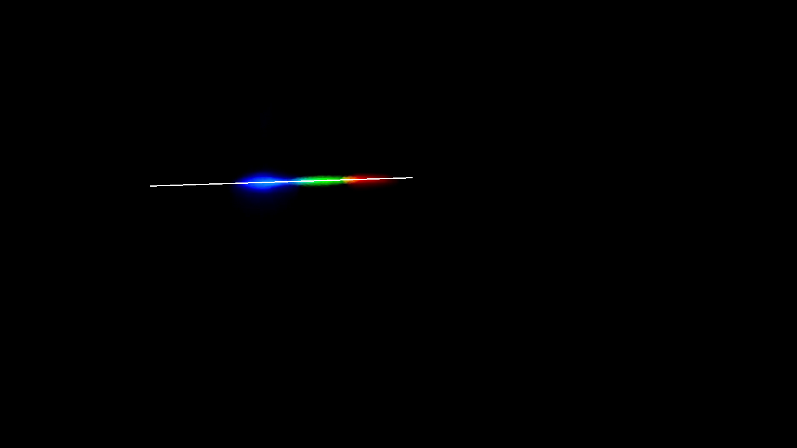
\includegraphics[width=0.4\textwidth]{data/calibration_curve.png}
    \caption{Reta de calibração $\lambda(x) = -0.0608250474x + 203.136815$ ajustada via regressão linear. Fonte: \cite{autoria_propria}.}
    \label{fig:calib_curve}
\end{figure}

% (3) Validação com Amostras Reais:
% \label{subsec:validacao}

% Um experimento de diluição de glicerina em água (faixa: 5–30\% v/v) foi realizado para validar o sistema. O espectro de absorção (Fig. \ref{fig:glicerina_verde}, Fig. \ref{fig:glicerina_vermelho} e Fig. \ref{fig:glicerina_azul}) mostrou picos característicos:

% \begin{equation}
%     R^2 = 0.94 \quad \text{(Correlação entre dados experimentais e teóricos)}
% \end{equation}

% \begin{figure}[ht]
%     \centering
%     \begin{subfigure}{0.32\textwidth}
%         \centering
%         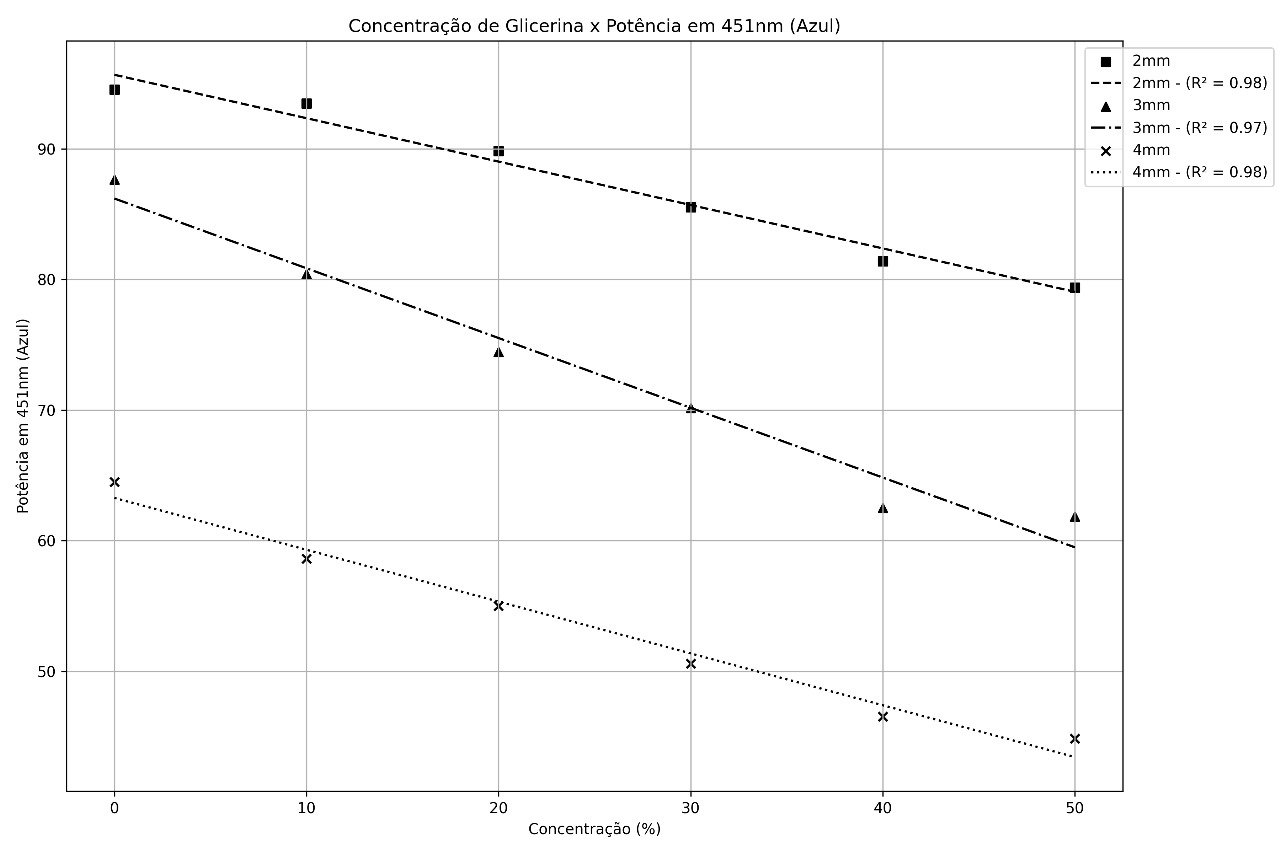
\includegraphics[width=\textwidth]{data/glicerina_spectrum_azul.jpeg}
%         \caption{LED azul}
%         \label{fig:glicerina_azul}
%     \end{subfigure}
%     \begin{subfigure}{0.32\textwidth}
%         \centering
%         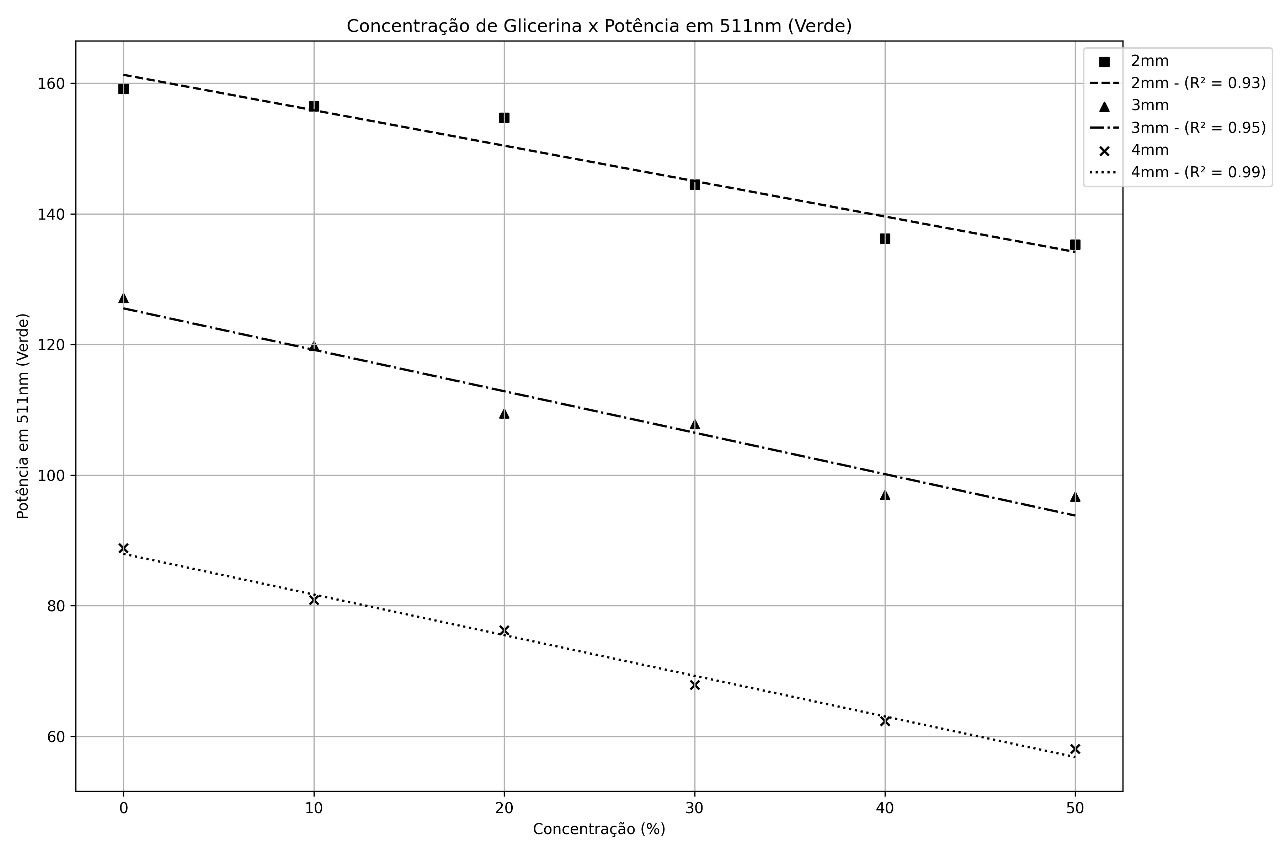
\includegraphics[width=\textwidth]{data/glicerina_spectrum_verde.jpeg}
%         \caption{LED verde}
%         \label{fig:glicerina_verde}
%     \end{subfigure}
%     \begin{subfigure}{0.32\textwidth}
%         \centering
%         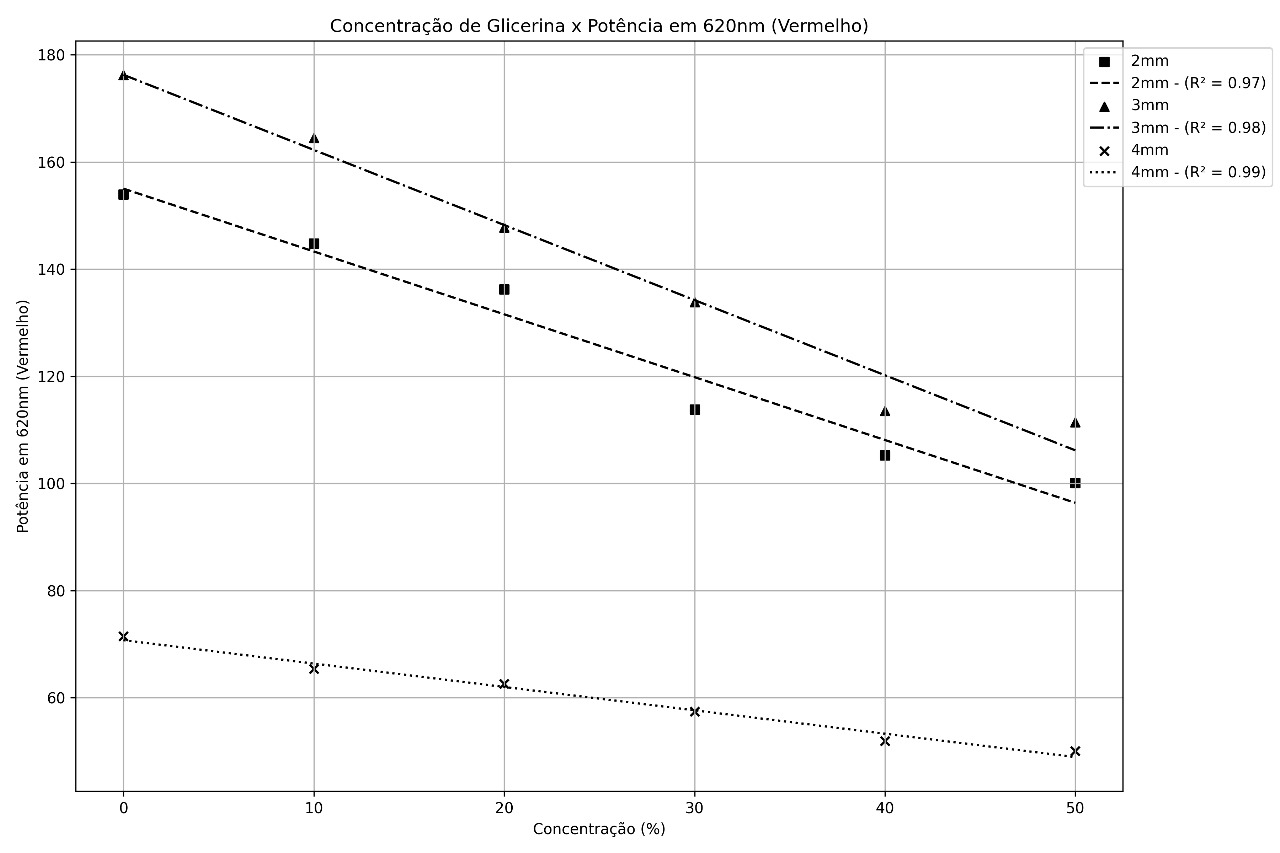
\includegraphics[width=\textwidth]{data/glicerina_spectrum_vermelho.jpeg}
%         \caption{LED vermelho}
%         \label{fig:glicerina_vermelho}
%     \end{subfigure}
%     \caption{Espectro de absorção de glicerina diluída em água em diferentes concentrações (5\%, 15\%, 30\%) para as fontes de luz LED azul, verde e vermelho.}
%     \label{fig:glicerina_espectros}
% \end{figure}

(3) Validação com Amostras Reais:
\label{subsec:validacao}

Um experimento de diluição de glicerina em água (faixa: 10–30\%) foi realizado para validar o sistema. O espectro de absorção (Fig. \ref{fig:glicerina_espectros}) mostrou picos característicos em 511 nm (verde) e 620 nm (vermelho), com alta correlação entre os dados experimentais e teóricos. Os coeficientes de determinação (\(R^2\)) para cada comprimento de onda foram:

\begin{itemize}
    \item \textbf{LED Verde}:
    \begin{itemize}
        \item 2 mm: \(R^2 = 0.93\)
        \item 3 mm: \(R^2 = 0.95\)
        \item 4 mm: \(R^2 = 0.99\)
    \end{itemize}
    \item \textbf{LED Vermelho}:
    \begin{itemize}
        \item 2 mm: \(R^2 = 0.97\)
        \item 3 mm: \(R^2 = 0.98\)
        \item 4 mm: \(R^2 = 0.99\)
    \end{itemize}
    \item \textbf{LED Azul}:
    \begin{itemize}
        \item 2 mm: \(R^2 = 0.98\)
        \item 3 mm: \(R^2 = 0.97\)
        \item 4 mm: \(R^2 = 0.98\)
    \end{itemize}
\end{itemize}

\begin{figure}[ht]
    \centering
    \begin{subfigure}{0.38\textwidth}
        \centering
        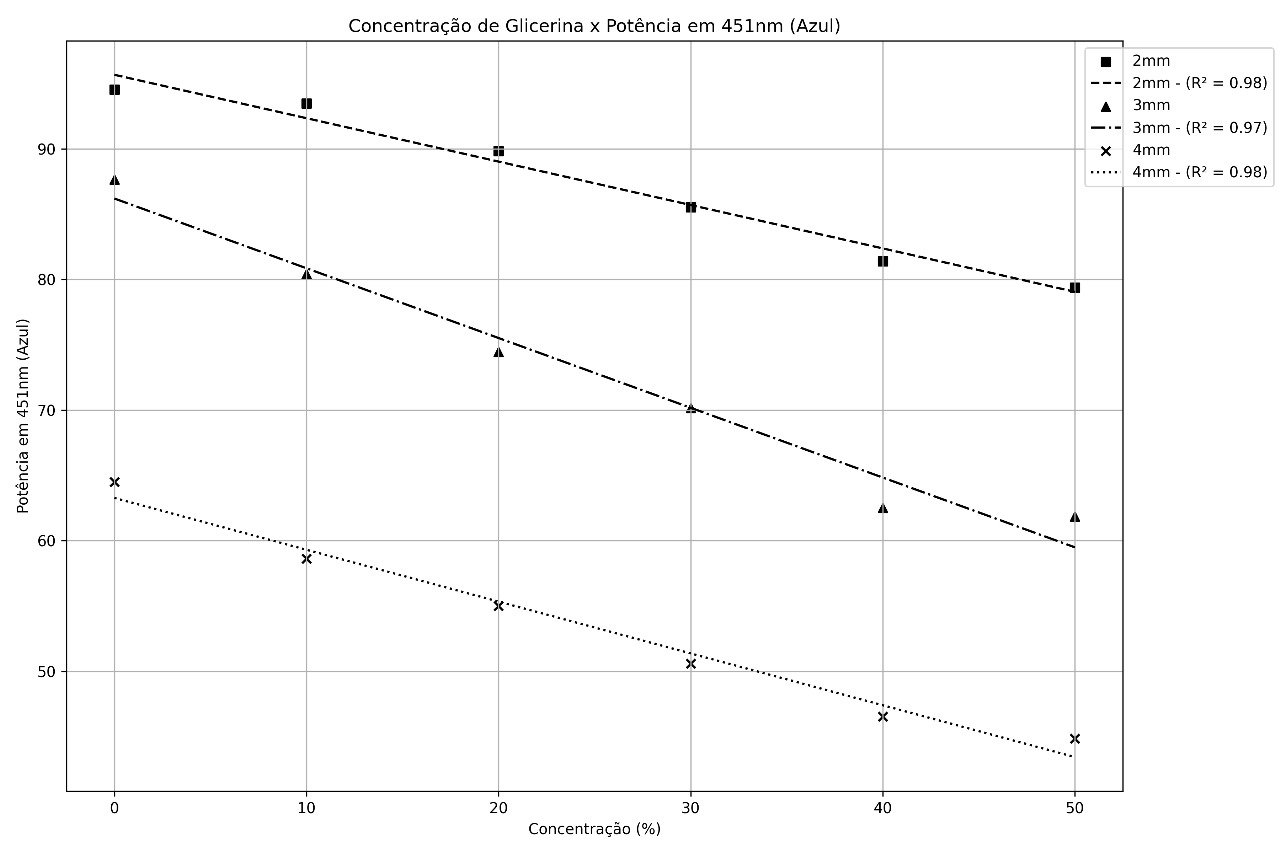
\includegraphics[width=\textwidth]{data/glicerina_spectrum_azul.jpeg}
        \caption{LED azul}
        \label{fig:glicerina_azul}
    \end{subfigure}
    \begin{subfigure}{0.38\textwidth}
        \centering
        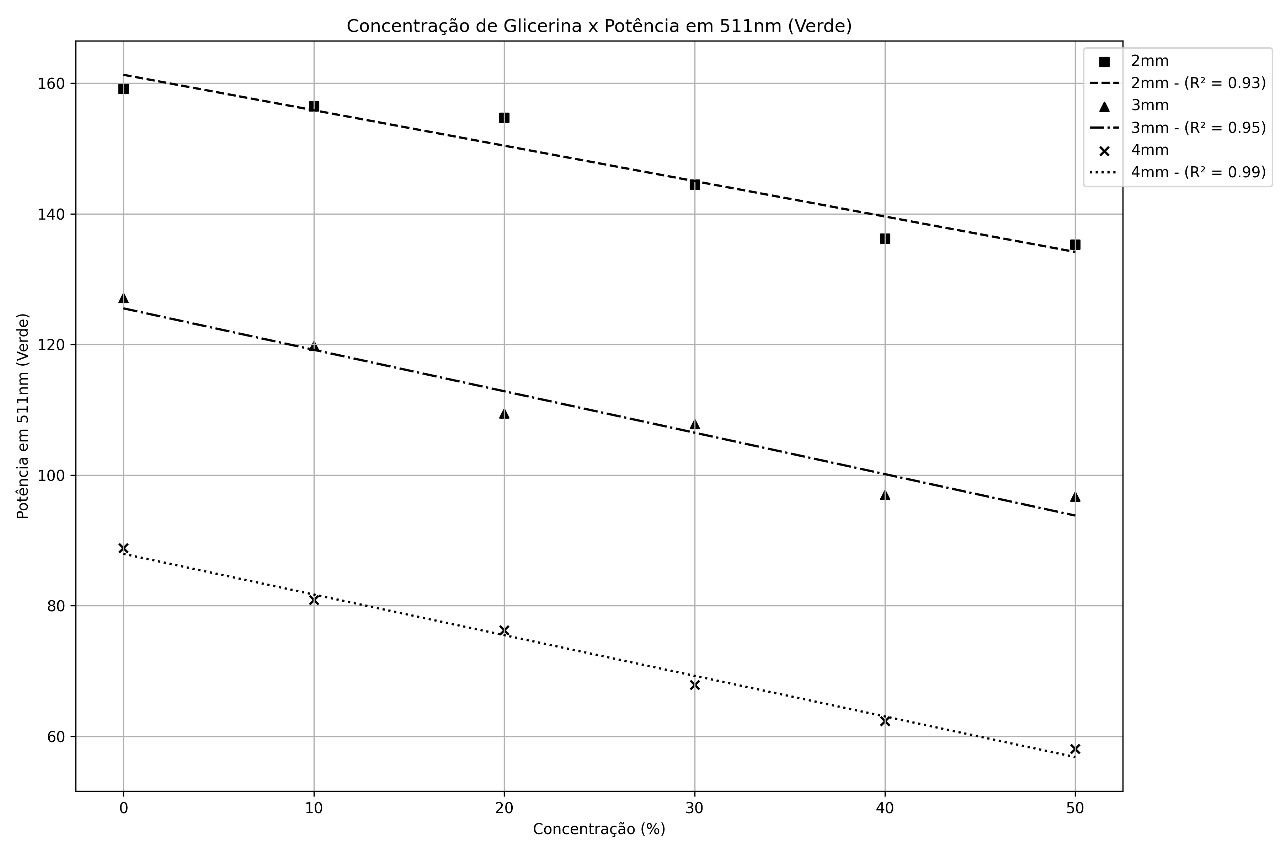
\includegraphics[width=\textwidth]{data/glicerina_spectrum_verde.jpeg}
        \caption{LED verde}
        \label{fig:glicerina_verde}
    \end{subfigure}
    \begin{subfigure}{0.38\textwidth}
        \centering
        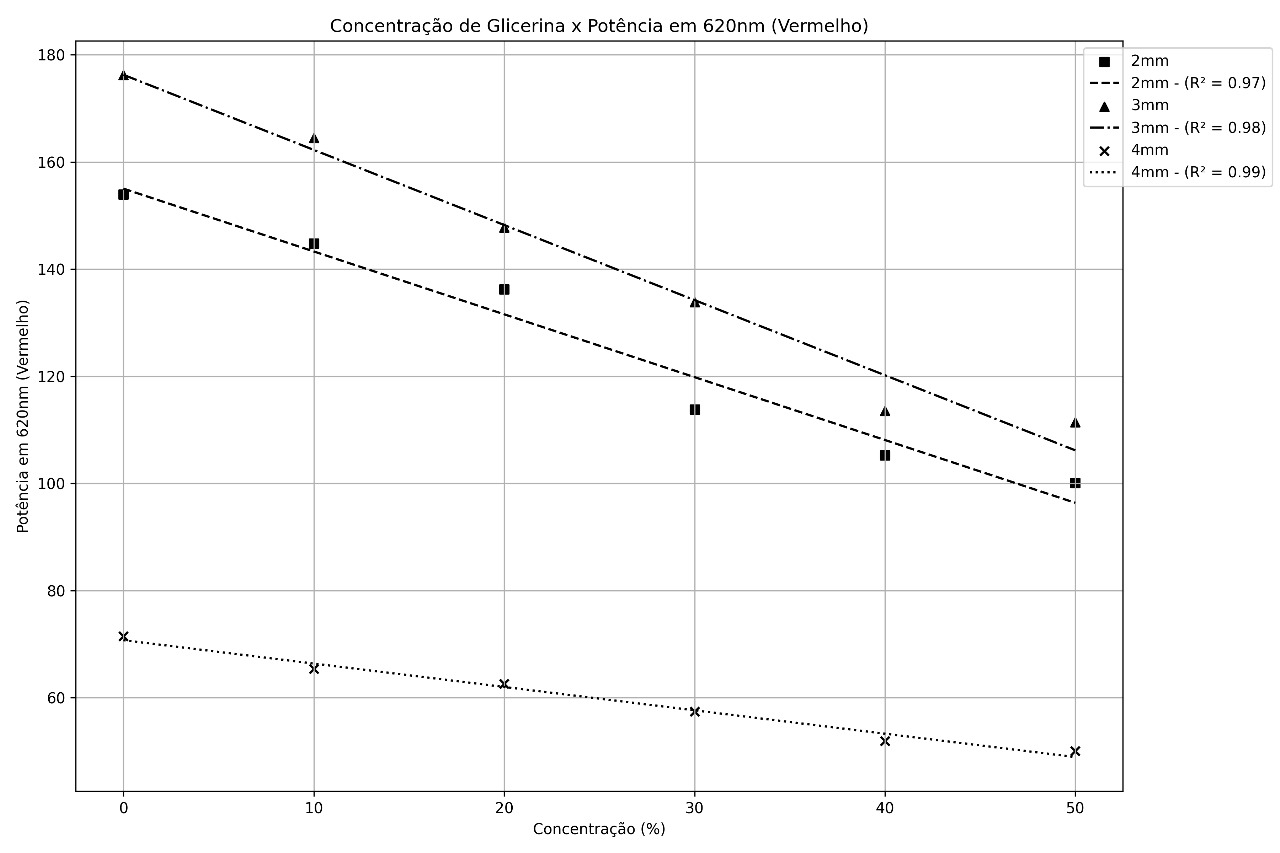
\includegraphics[width=\textwidth]{data/glicerina_spectrum_vermelho.jpeg}
        \caption{LED vermelho}
        \label{fig:glicerina_vermelho}
    \end{subfigure}
    \caption{Espectro de absorção de glicerina diluída em água em diferentes concentrações (10\%, 20\%, 30\%) para as fontes de luz LED azul, verde e vermelho. Fonte: \cite{autoria_propria}.}
    \label{fig:glicerina_espectros}
\end{figure}

% \subsection{Análise de Desempenho}
% O tempo total de calibração automatizada foi de $3.2 \pm 0.5$ minutos, contra $15$ minutos em métodos manuais \cite{zhang2020}. A Tabela \ref{tab:performance} resume o desempenho:

% \begin{table}[ht]
%     \centering
%     \caption{Desempenho do sistema OSA Visível}
%     \label{tab:performance}
%     \begin{tabular}{lcc}
%         \toprule
%         Métrica & Valor \\
%         \midrule
%         Precisão (RMS) & $\pm 1.8$ nm \\
%         Tempo de processamento por quadro & 12 ms \\
%         Resolução espacial & 0.5 nm/pixel \\
%         Consumo de memória & 45 MB \\
%         \bottomrule
%     \end{tabular}
% \end{table}

\section{CONCLUSÃO}  
\label{sec:conclusao}  

Este trabalho demonstrou a viabilidade de um Analisador de Espectro Óptico (OSA) de baixo custo para a faixa visível (380–750 nm), integrando hardware acessível (\textit{Osinha}) e software customizado (\textit{OSA Visível}). O sistema proposto alcançou uma precisão de $\pm 1.8$ nm na calibração automatizada, validada experimentalmente por meio de lasers de referência (532 nm e 650 nm) e ensaios com diluição de glicerina em água (10–30\%), onde se observou alta correlação ($R^2 \geq 0.93$) entre dados experimentais e teóricos (Fig. \ref{fig:glicerina_espectros}).  

A abordagem de calibração híbrida — combinando regressão linear com luz branca e ajuste absoluto via lasers — superou as limitações de métodos manuais ou dependentes de hardware dedicado. A solução proposta reduziu custos em mais de 98\% em comparação a sistemas comerciais (Tabela \ref{tab:market}), com um custo total inferior a \$200 USD, tornando-a acessível para instituições educacionais e laboratórios de pequeno porte.  

Como próximos passos, destacam-se:  
\begin{itemize}  
    \item Incorporação de modelos não lineares para aprimorar a precisão em extremos do espectro (e.g., abaixo de 400 nm e acima de 700 nm).  
    \item Expansão da faixa espectral para o infravermelho próximo (750–1100 nm), utilizando sensores CMOS otimizados.  
    \item Desenvolvimento de uma plataforma \textit{Software as a Service} (SaaS) para acesso remoto e análise de dados em tempo real via web.
\end{itemize}  

A interface intuitiva do \textit{OSA Visível}, aliada à automação inteligente do processo de calibração, reforça o potencial do sistema como ferramenta versátil para aplicações em automação óptica, educação e pesquisa de baixo custo. 

\section{AGRADECIMENTOS}  
Agradecemos ao Laboratório LITel/UFJF pelo suporte infraestrutural e aos orientadores pelo acompanhamento técnico. Reconhecemos também o apoio da Universidade Federal de Juiz de Fora (UFJF) pelo fomento à iniciação científica. Este trabalho foi financiado pelas agências de fomento FAPEMIG, CNPq e CAPES, cujo apoio foi fundamental para o desenvolvimento desta pesquisa. 

% (Adicione agências de fomento, se aplicável, ex: À FAPEMIG pelo financiamento via edital XX/2023.)  

\bibliography{ifacconf}             % bib file to produce the bibliography
                                                     % with bibtex (preferred)
                                                   
%\begin{thebibliography}{xx}  % you can also add the bibliography by hand

%\bibitem[Able(1956)]{Abl:56}
%B.C. Able.
%\newblock Nucleic acid content of microscope.
%\newblock \emph{Nature}, 135:\penalty0 7--9, 1956.

%\bibitem[Able et~al.(1954)Able, Tagg, and Rush]{AbTaRu:54}
%B.C. Able, R.A. Tagg, and M.~Rush.
%\newblock Enzyme-catalyzed cellular transanimations.
%\newblock In A.F. Round, editor, \emph{Advances in Enzymology}, volume~2, pages
%  125--247. Academic Press, New York, 3rd edition, 1954.

%\bibitem[Keohane(1958)]{Keo:58}
%R.~Keohane.
%\newblock \emph{Power and Interdependence: World Politics in Transitions}.
%\newblock Little, Brown \& Co., Boston, 1958.

%\bibitem[Powers(1985)]{Pow:85}
%T.~Powers.
%\newblock Is there a way out?
%\newblock \emph{Harpers}, pages 35--47, June 1985.

%\bibitem[Soukhanov(1992)]{Heritage:92}
%A.~H. Soukhanov, editor.
%\newblock \emph{{The American Heritage. Dictionary of the American Language}}.
%\newblock Houghton Mifflin Company, 1992.

%\end{thebibliography}

% \appendix
% \section{Sumário da gramática sânscrita}    % Each appendix must have a short title.
% \section{Algum vocabulário maia}              % Sections and subsections are supported  
%                                                                          % in the appendices.
\end{document}
